\documentclass{article}[12pt]
\usepackage{silence}
\usepackage{graphicx}
\usepackage{hyperref}

\hbadness=9999999

\newcommand{\aetitle}{WortEx} % Title of the report
\newcommand{\studentOne}{Artur Schäfer} % Name 1
\newcommand{\studentTwo}{Donatien Leray} % Name 2

\begin{document}
\noindent
Linguistic gaming with Python \hfill \studentOne\\
WS 23/24 \hfill \studentTwo

\vspace{1cm}

\begin{figure}[ht]
    \centering
    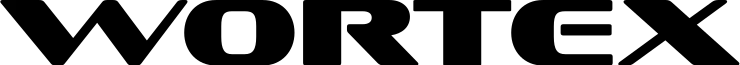
\includegraphics[width=250pt,height=33pt]{pictures/logo_black.png}
\end{figure}

\vspace{0.5cm}

    \section*{Introduction}

    Leaning new words can be pretty boring, so we have created a game to make
    it more exciting. Wortex is a linguistic word game. It is designed to
    challenge players' linguistic skills by letting them write all the words
    they can form out of a given set of letters. Linguistic
    games offer a fun way to improve vocabulary and spelling skills and learn new words.

    \section*{Objectives}

    The primary objective of Wortex is to form as many words as possible from a
    given set of seven letters. Players must create words of at least three
    letters, up  to the maximum length of seven. \\ The more words a player
    forms, the higher their score. To achieve a top score, players should aim
    to construct not only words, that are as long as possible but also rare. More about that in \nameref{Scoring}.
    The game ends if the timer runs out or if the player finds all possible
    words, that can be formed from the set of given letters.

    \section*{Features}

    \subsection*{Menu}

    Upon launching Wortex, players are presented with a menu. Here, they can
    choose a language (English or German) they prefer to play with. More languages can be added, see \nameref{Adding_a_new_language} There is also
    a button to view a scoreboard, which is showcasing the highest scores ever
    achieved in a specific difficulty level. The player can choose between four of them in the main menue befor playing. The default difficulty is the lowest "easy" wich gives the player 2 min time followed by "medium" (60s), "hard" (30s) and finaly "extreme" with only 15s time.
    \newpage

    \begin{figure}[ht]
        \centering
        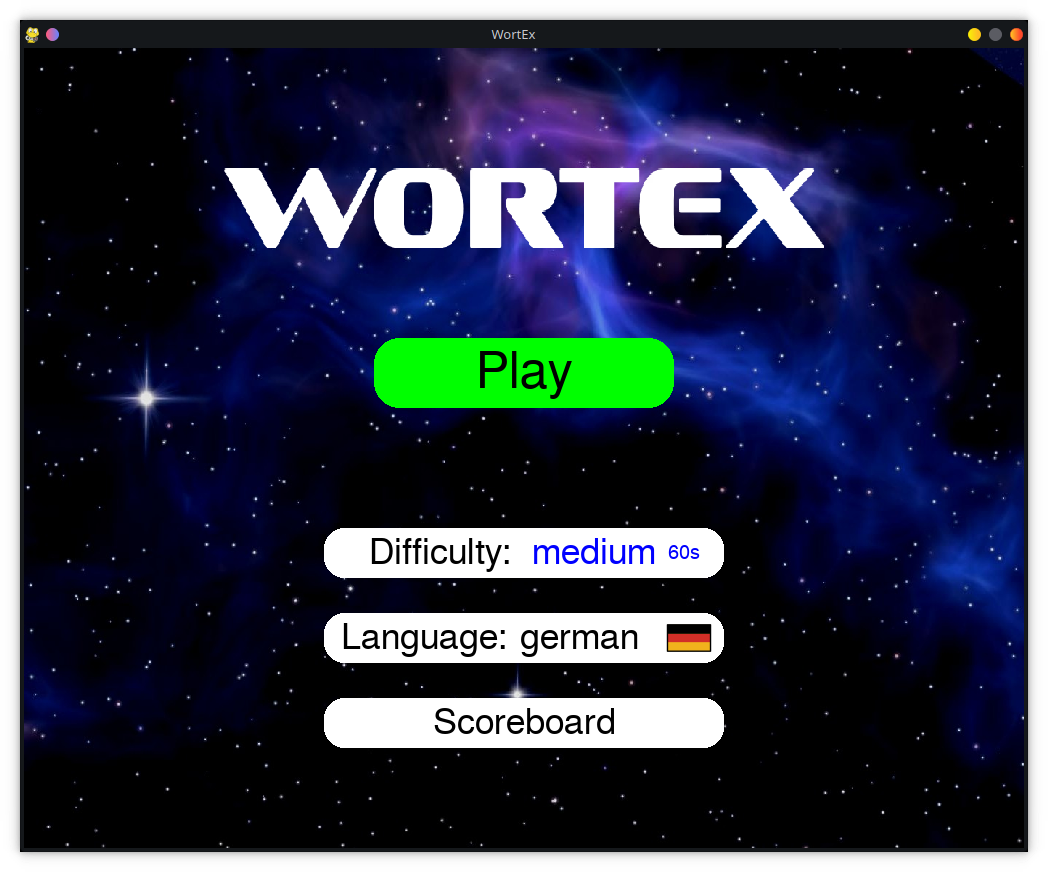
\includegraphics[width=0.5\textwidth]{pictures/menu.png}
        \caption{The main menu of Wortex}
    \end{figure}

    \subsection*{Game}

    Upon starting the game, you can
    see a timer, the score, and a list of words that appears if the player
    types a correct word. In the middle there is a circle that represents the
    time and in that circle there are the letters that can be typed to form
    words. Also, there is information about how many words can be found in the
    given set. The player can create the words by typing the letters on the
    keyboard. With the escape, return or enter key, the player can reset his input or delete the last letter with backspace.\\
    After guessing a correct word, the input gets cleared and the found word is
    added to the list of found words.\\ If a seven-letter word is found, the
    player gets bonus time (10 seconds) to find more words. There are no penalties for guessing wrong. The player is just wasting
    time that could have been used to find more words. 

       \begin{figure}[h!]
        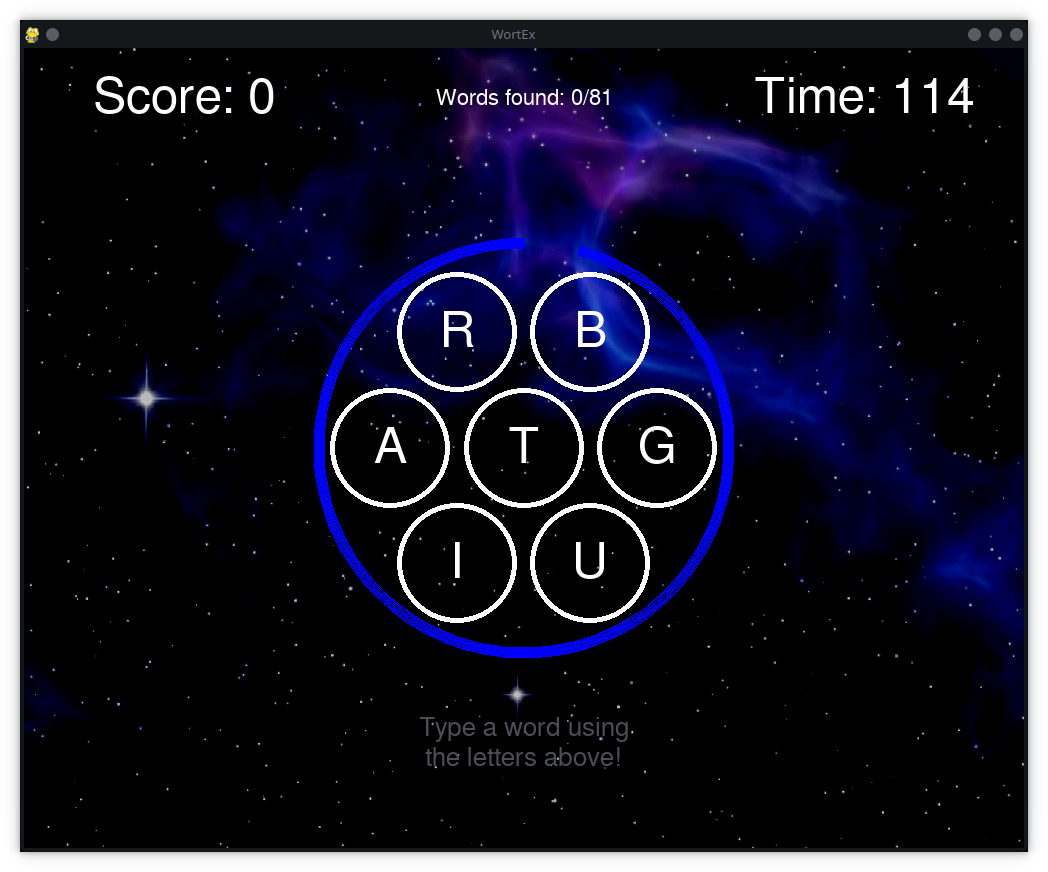
\includegraphics[width=0.49\textwidth]{pictures/gameplay.png}
        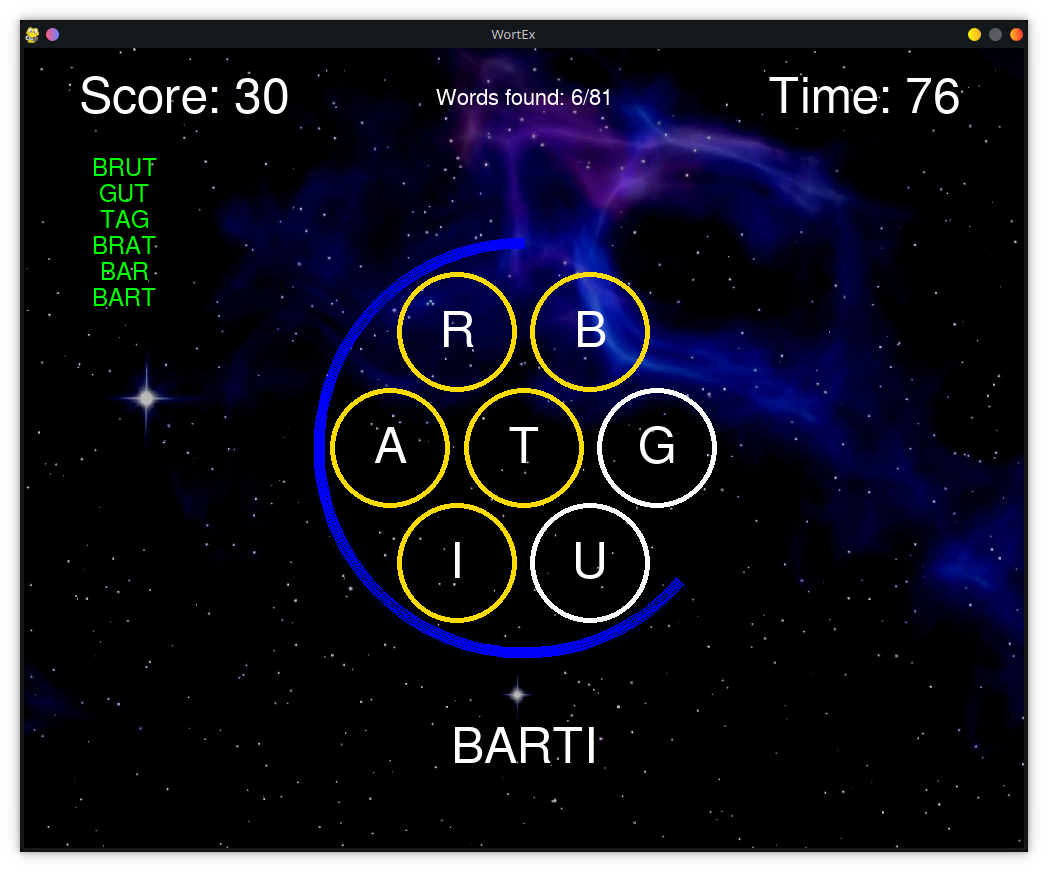
\includegraphics[width=0.49\textwidth]{pictures/mid_game.png}
        \caption{Gameplay of Wortex}
    \end{figure}
    
    \newpage

    \subsection*{Endscreen}
    
    After the timer runs out or the player achieves to find all possible words,
    the game ends, and the player is presented with a endscreen that shows the
    score. If the player made it to the scoreboard (top 10) he will be notified about it same if a new highscore was achieved.\\ All the words that could be found are displayed on the endscreen. The words that were found are highlighted green. All of them can be clicked to open a definition of them in the browser. In German, we open the online Duden
    dictionary and for English, the online Oxford Dictionary. The player can
    start a new game by pressing the play again button, or go back to the
    main menu. 

    \begin{figure}[h!]
        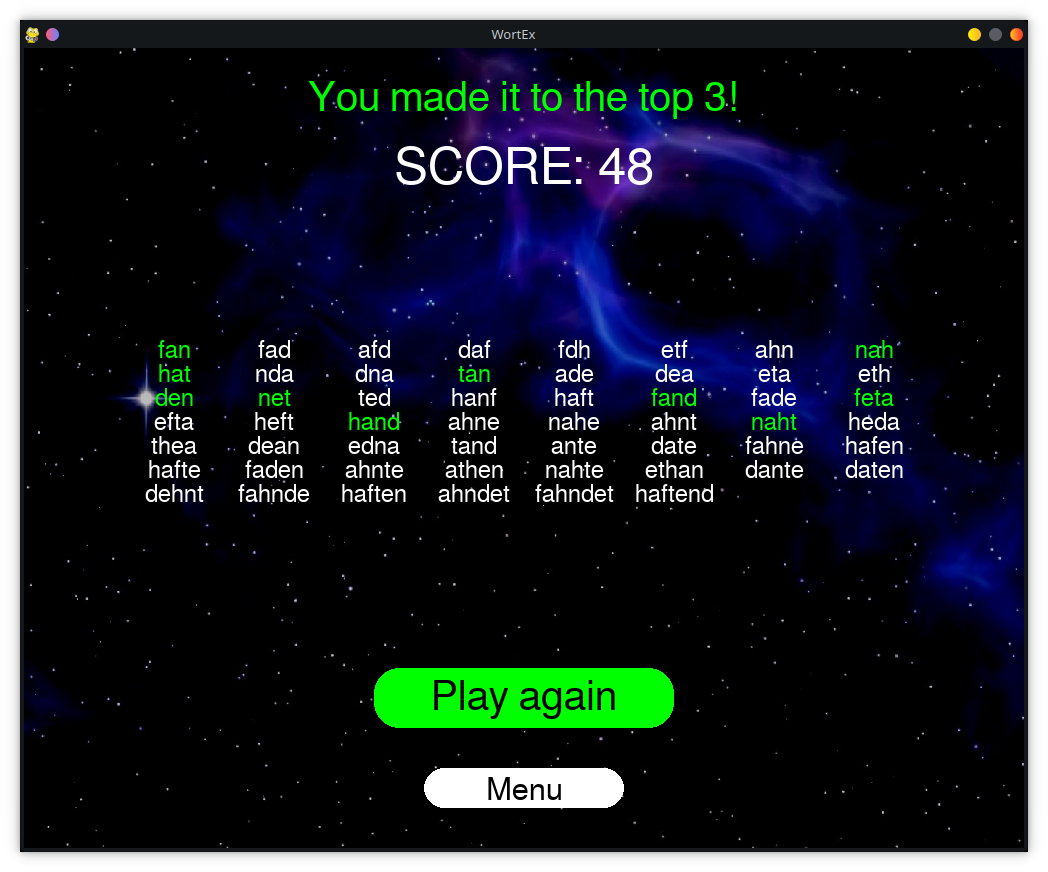
\includegraphics[width=0.49\textwidth]{pictures/endcard.png}
        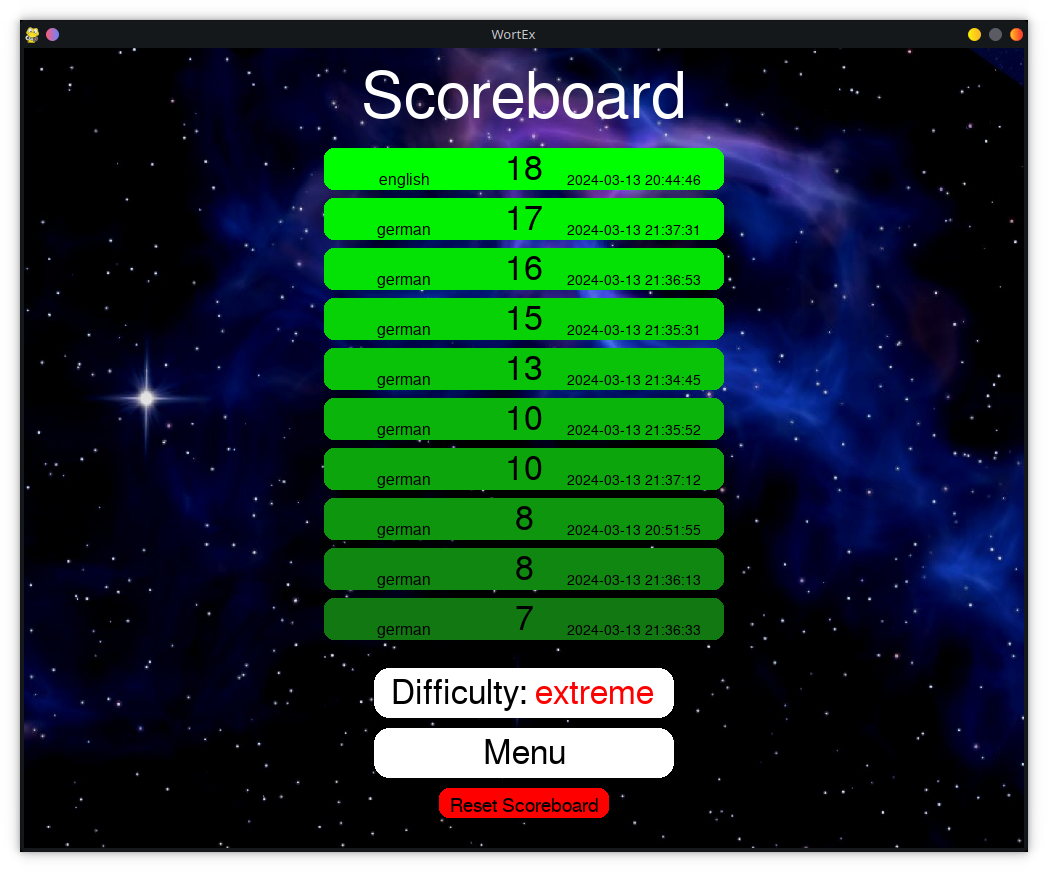
\includegraphics[width=0.49\textwidth]{pictures/scoreboard.png}
        \caption{The Endscreen and Scoreboard}
    \end{figure}

    \subsection*{Scoreboard}
    From the main menu the player can view a leaderboard, which
    shows the 10 highest scores ever achieved in a given difficulty.
    The score are depicted along with a timestamp and information in which language they were achieved. To cycle through the scoreboards just press the difficulty button. The top 10 scores for each difficulty are saved in the database. The scores can be reset with the reset button.

    \subsection*{The Database}

    It is very frustrating to find a word the game doesn't recognize.
    To work against that, we want our dataset to be as big as possible while still staying fast. Calculating all answers for a given word is quite expensive, that's why it's preprocessed and stored in a database.\\\\
    We used a frequency list from a GitHub
    repository that contains about $\sim$ 7.500.00 words and their frequency in the
    German language. This data contains a lot of noise that needs to be cleaned. We filtered all the words that are out of range of 3 to 7
    letters or contain letters that are not German. Then names are filtered out and only the words that can be double-checked with a dictionary of roughly 60.000 words are kept. Resulting in about 40.000 valid words.
    From these we get all seven-letter words. Because the order of the letters doesn't matter, anagrams would give exactly the same answers, so we filter these out. Finally, we calculate all possible answers and their corresponding points and save them in the database, taking the original seven-letter word as key.


    \subsection*{Scoring}\label{Scoring}

    The score is calculated by the length the frequency of the word of that
    given language. Frequency describes how often a word appears in a large
    amount of text. The more frequent a word is, the fewer points the player
    gets for guessing that word.
    The points a word gives is calculated given following formula:
    \begin{equation}
       p_i = 1 + \frac{(L(i) - 2) \cdot (1 + 10 \cdot (1 - F_{rel}(i)))}{15} 
    \end{equation}
    \noindent
    $p_i$ are the points of a word $i$, $L(i)$ is the length of that word and $F_{rel}$
    is the relative frequency of it. The relative frequency of a word is calculated by dividing the highest frequency by the frequency of the given word $F_{rel}(i)=\frac{F_{max}}{F_{i}}$. For the most common $F_{rel}=1$ and a word that is half as common will have $F_{rel}=0,5$.\\
    The points are then multiplied by a factor that is
    calculated by the average points of all words. This factor is used to make
    the points more accurate. Less possible words or harder words will increase the points given. 
    \begin{equation}
        f = \frac{\sum_{i=1}^{n} p_i}{n}
    \end{equation}
    We finally round the points and return them as an integer.
    \begin{equation}
        P_i = \left\lfloor p_i \cdot f \right\rfloor
    \end{equation}
    
    \subsection*{Easter Eggs}

    If the player manages to form the words "Wortex", "Dodo" or "Artur" they
    receive a bonus of 42 points and gain 10 seconds. Also, the look of the game
    changes a bit.

    \subsection*{Adding a new language}\label{Adding_a_new_language}
    It is possible to easily add languages if you have a compatible frequency list. How this works is described in greater details in the \href{https://github.com/donatienLeray/WortEx#add-your-own-language}{README}

\end{document}
